\documentclass{article}

\usepackage{fancyhdr}
\usepackage{extramarks}
\usepackage{amsmath}
\usepackage{amsthm}
\usepackage{amssymb}
\usepackage{amsfonts}
\usepackage[plain]{algorithm}
\usepackage{algpseudocode}
\usepackage{enumitem}
\usepackage{hyperref}
\usepackage{changepage}
\usepackage{graphicx}
\usepackage{listings}
\usepackage[dvipsnames]{xcolor}

%
% Basic Document Settings
%

\topmargin=-0.45in
\evensidemargin=0in
\oddsidemargin=0in
\textwidth=6.5in
\textheight=9.0in
\headsep=0.25in

\linespread{1.1}

\pagestyle{fancy}
\lhead{\hmwkAuthorName}
\chead{\hmwkClass\ (\hmwkClassInstructor\ \hmwkClassTime): \hmwkTitle}
\rhead{\firstxmark}
\lfoot{\lastxmark}
\cfoot{\thepage}

\renewcommand\headrulewidth{0.4pt}
\renewcommand\footrulewidth{0.4pt}

\setlength\parindent{0pt}

% Create Problem Sections
%

\newcommand{\enterProblemHeader}[1]{
    \nobreak\extramarks{}{Problem \arabic{#1} continued on next page\ldots}\nobreak{}
    \nobreak\extramarks{Problem \arabic{#1} (continued)}{Problem \arabic{#1} continued on next page\ldots}\nobreak{}
}

\newcommand{\exitProblemHeader}[1]{
    \nobreak\extramarks{Problem \arabic{#1} (continued)}{Problem \arabic{#1} continued on next page\ldots}\nobreak{}
    \stepcounter{#1}
    \nobreak\extramarks{Problem \arabic{#1}}{}\nobreak{}
}

\setcounter{secnumdepth}{0}
\newcounter{partCounter}
\newcounter{homeworkProblemCounter}
\setcounter{homeworkProblemCounter}{1}
\nobreak\extramarks{Problem \arabic{homeworkProblemCounter}}{}\nobreak{}

%
% Homework Problem Environment
%
% This environment takes an optional argument. When given, it will adjust the
% problem counter. This is useful for when the problems given for your
% assignment aren't sequential. See the last 3 problems of this template for an
% example.
%
\newenvironment{homeworkProblem}[1][-1]{
    \ifnum#1>0
        \setcounter{homeworkProblemCounter}{#1}
    \fi
    \section{Problem \arabic{homeworkProblemCounter}}
    \setcounter{partCounter}{1}
    \enterProblemHeader{homeworkProblemCounter}
}{
    \exitProblemHeader{homeworkProblemCounter}
}

%
% Homework Details
%   - Title
%   - Due date
%   - Class
%   - Section/Time
%   - Instructor
%   - Author
%

\newcommand{\hmwkTitle}{PA\ \#2}
\newcommand{\hmwkDueDate}{April 1, 2016}
\newcommand{\hmwkClass}{CSE 489}
\newcommand{\hmwkClassTime}{T/TH 2:00-3:20PM}
\newcommand{\hmwkClassInstructor}{Dimitrios Koutsonikolas}
\newcommand{\hmwkAuthorName}{Robert Shannon}
\newcommand{\hmwkIntegrityStmt}{}

%
% Title Page
%

\title{
    \vspace{2in}
    \textmd{\textbf{\hmwkClass:\ \hmwkTitle}}\\
    \normalsize\vspace{0.1in}\small{Due\ on\ \hmwkDueDate\ at 2:00pm}\\
    \vspace{0.1in}\large{\textit{\hmwkClassInstructor\ \hmwkClassTime}}
    \vspace{3in}}

\author{\textbf{\hmwkAuthorName}}
\date{}

\renewcommand{\part}[1]{\textbf{\large Part \Alph{partCounter}}\stepcounter{partCounter}\\}

%
% Various Helper Commands
%

% Useful for algorithms
\newcommand{\alg}[1]{\textsc{\bfseries \footnotesize #1}}

% For derivatives
\newcommand{\deriv}[1]{\frac{\mathrm{d}}{\mathrm{d}x} (#1)}

% For partial derivatives
\newcommand{\pderiv}[2]{\frac{\partial}{\partial #1} (#2)}

% Integral dx
\newcommand{\dx}{\mathrm{d}x}

% Probability commands: Expectation, Variance, Covariance, Bias
\newcommand{\E}{\mathrm{E}}
\newcommand{\Var}{\mathrm{Var}}
\newcommand{\Cov}{\mathrm{Cov}}
\newcommand{\Bias}{\mathrm{Bias}}

% C++ Syntax Highlighting
\lstset{language=C++,
                keywordstyle=\color{blue},
                stringstyle=\color{red},
                commentstyle=\color{OliveGreen},
                morecomment=[l][\color{magenta}]{\#}
}

\begin{document}

\maketitle

\pagebreak

\section{Statement of Academic Integrity}
I have read and understood the course academic integrity policy located under this link:
\url{http://www.cse.buffalo.edu/faculty/dimitrio/courses/cse4589_s16/index.html\#integrity}

\section{Multiple Software Timers for Selective Repeat}
The Selective Repeat protocol requires an individual timer for each unacknowledged packet, but the simulator only provides a single hardware timer. To work around this constraint,
multiple software timers were implemented using the single hardware timer provided by the simulator. This was achieved by the following steps:
\begin{enumerate}
	\item Use a struct \colorbox{gray}{\lstinline[basicstyle=\ttfamily\color{white}]|<pkt_timer>|}
 to represent each software timer
	\item Set the hardware timer to fire every 1.0 second
	\item Fire all expired software timers each time a hardware timer interrupt occurs
	\item For each software timer interrupt, call the software timer interrupt handler routine
	\item After handling the software timer interrupt, restart the timer
	\item Repeat steps 3-5 until program exits
\end{enumerate}
\begin{lstlisting}[frame=single]
/**
 * A packet timer.
 */
struct pkt_timer {
  int seq_num;     // Sequence number of the packet associated with this timer
  float next_fire; // Next scheduled timer interrupt
  bool active;     // Whether this timer is active or not
};
/**
 * Container for all packet timers.
 */
std::vector<pkt_timer> pkt_timers;
/**
 * Helper methods to manage multiple packet timers
 * and their corresponding interrupt handlers.
 */
/* Create new packet timer */
void new_pkt_timer(int seq_num);
/* Destroy existing packet timer */
void destroy_pkt_timer(int seq_num);
/* Check if packet timer exists */
bool pkt_timer_exists(int seq_num);
/* Trigger a packet timer interrupt */
void fire_pkt_timer(int seq_num);
/* Default packet timer interrupt handler routine */
void pkt_timer_interrupt_handler(int seq_num);
/* Fire interrupt for all expired packet timers */
void fire_expired_pkt_timers();
\end{lstlisting}

\pagebreak

\section{Timeout Schemes Used}
The timeout interval (how long a protocol waits before resending unacknowledged packet(s)) was chosen to maximize throughput performance with an application generating messages every 50 time units under the widest range of conditions possible. The ``optimal'' values below were determined through experimentation, with foreknowledge of the RTT time to be on average 10.0 time units. 

\begin{enumerate}
    \item \textbf{Alternating Bit (ABT)} --- $t=10.0$, re-send unacknowledged packet after 10.0 time units.
    \item \textbf{Go-Back-N (GBN)} --- $t=11.0$, re-send all unacknowledged packets after 11.0 time units.
    \item \textbf{Selective-Repeat (SR)} --- $t=15.0$, re-send unacknowledged packet after 15.0 time units. Note that SR uses an individual timer for each unacknowledged packet.
\end{enumerate}

All of the timeout values are very close (or equal to in the case of ABT) to the link's average RTT. This is because the average RTT is the expected amount of time to receive an ACK after sending a packet. If an ACK is not received within 1 RTT, it is assumed that the corresponding packet or the ACK itself were either lost or corrupted, and as a result needs to be re-sent.

\pagebreak

\section{Experiments}

In each of the experiments below, the protocols were tested by sending 1,000 messages from sender to receiver, with a mean time of 50 time units between message arrivals, and a corruption probability of 0.2. The window sizes and loss probabilities were varied as specified, and the resulting throughput of each protocol plotted.

\subsubsection{1.a. Window size: 10; X-axis: Loss probability; Y-axis: Throughput (ABT, GBN and SR)}

\begin{center}
    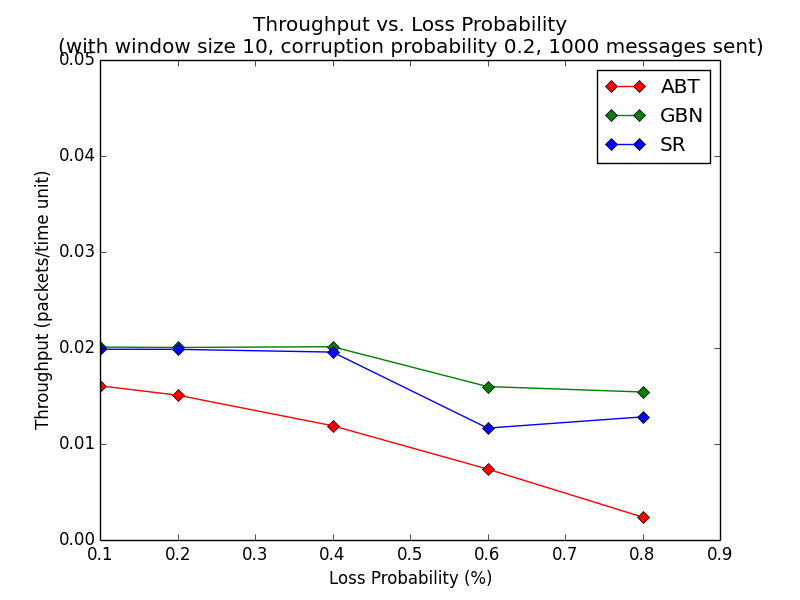
\includegraphics[width=330pt,height=245pt]{images/exp1g1.png}
\end{center}

\textbf{Expected}: Throughput to decrease as loss probability increases. Similar throughput performance of both SR and GBN (with SR utilizing the link more efficiently). Inferior throughput performance of ABT when compared to SR and GBN across a wide range of loss probabilities. 
\newline\newline
\textbf{Observed}: Increasing loss probability lowers throughput. The maximum throughput of both SR and GBN are about equal with this window size. SR's throughput drops lower than that of GBN's at a loss probability at roughly $l\ge0.6$. Both SR and GBN maintain their maximum throughput through $0.1 \le l \le 0.4$, while ABT's throughput drops consistently as loss probability is increased.
\newline\newline
\textbf{Conclusion}: Increased packet loss eventually decreases throughput. SR and GBN appear to be more resilient to packet loss than ABT.

\pagebreak

\subsubsection{1.b. Window size: 50; X-axis: Loss probability; Y-axis: Throughput (ABT, GBN and SR)}

\begin{center}
    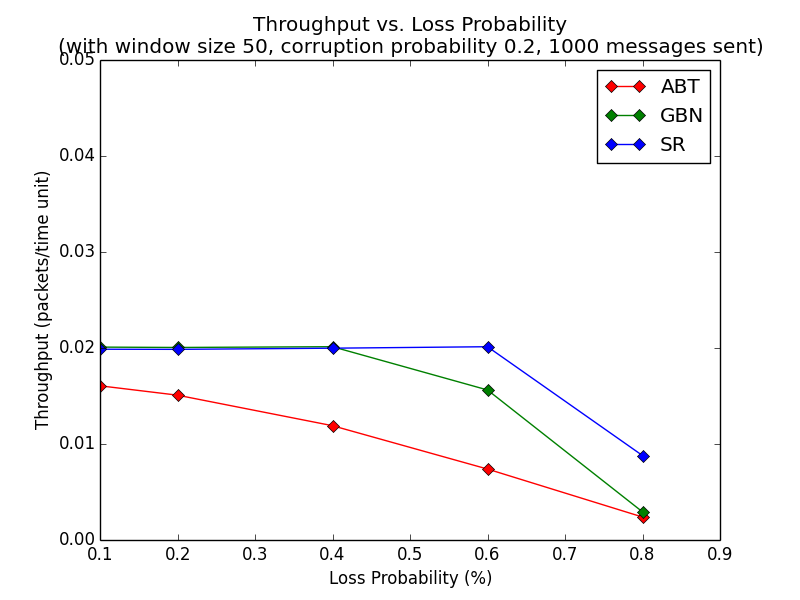
\includegraphics[width=330pt,height=245pt]{images/exp1g2.png}
\end{center}

\textbf{Expected}: Same results as experiment (1a), but more throughput for SR and GBN with a larger window size.
\newline\newline
\textbf{Observed}: Throughput drops with $t\ge0.6$ for SR, and $t\ge0.4$ for GBN. SR can maintain maximum throughput with up to 60\% packet loss, while GBN can only do so with up to 40\% packet loss. SR has a throughput that is consistently greater than or equal to that of GBN. ABT is again outperformed by both GBN and SR under all packet loss scenarios.
\newline\newline
\textbf{Conclusion}: The larger window size did not result in more throughput, likely because the sender was not sending messages fast enough to fill the pipeline. Interestingly, increasing the window size made SR more resilient to packet loss while maintaining maximum throughput. SR at least matches or outperforms GBN in terms of throughput at most levels of packet loss.

\pagebreak

\subsubsection{2.a. Loss probability: 0.2; X-axis: Window size; Y-axis: Throughput (ABT, GBN and SR)}

\begin{center}
    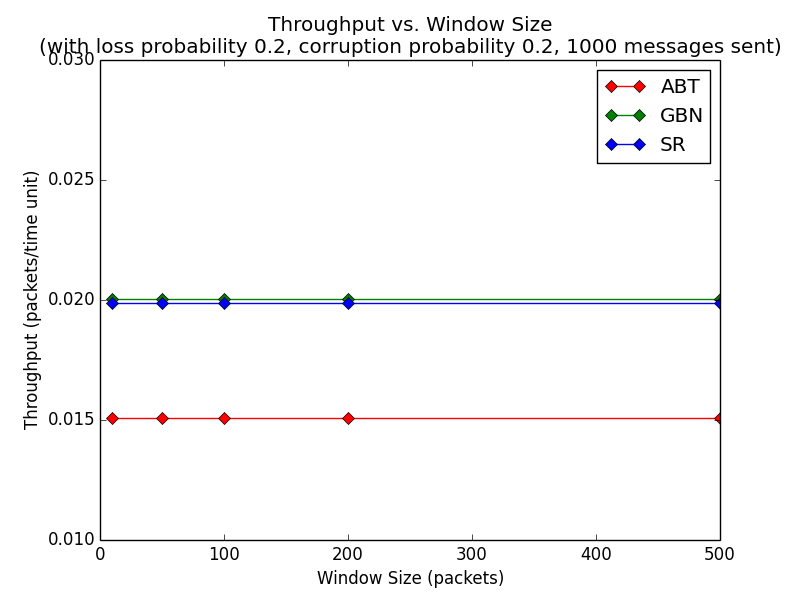
\includegraphics[width=330pt,height=245pt]{images/exp2g1.png}
\end{center}

\textbf{Expected}: Constant throughput amongst all three protocols, with GBN and SR offering the highest throughput and ABT the lowest. ABT to most certainly be constant because it does not make use of windows.
\newline\newline
\textbf{Observed}: All three protocols have a constant throughput across all window sizes.
\newline\newline
\textbf{Conclusion}: A larger window will increase throughput only if an application is sending messages fast enough to fill it. Since SR and GBN both use windows, their maximum throughput is the same when packet loss is minimal.

\pagebreak

\subsubsection{2.b. Loss probability: 0.5; X-axis: Window size; Y-axis: Throughput (ABT, GBN and SR)}

\begin{center}
    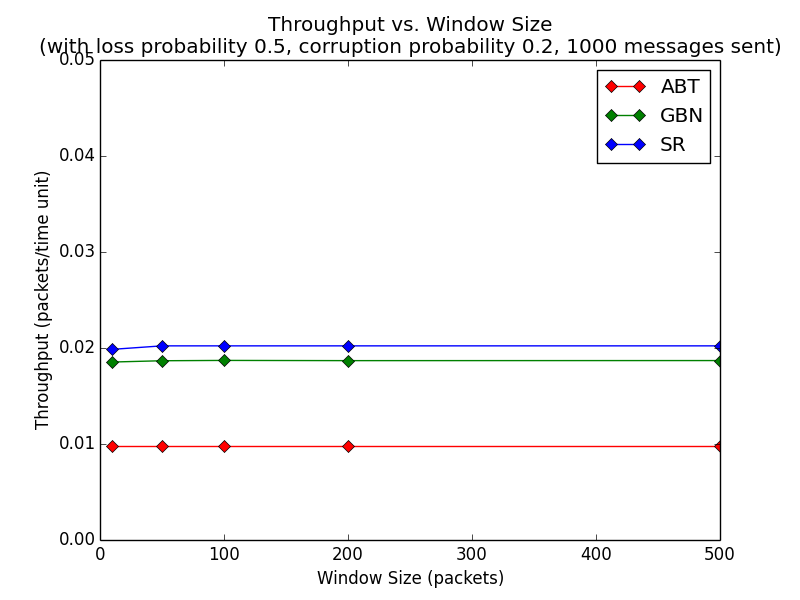
\includegraphics[width=330pt,height=245pt]{images/exp2g2.png}
\end{center}

\textbf{Expected}: Constant throughput for each protocol, but lower than than that of experiment (2a) due to increased packet loss.
\newline\newline
\textbf{Observed}: A performance regression with window size 10 for SR at this level of packet loss. At larger window sizes $\ge 50$, all three protocols again have a constant throughput, but this time SR clearly outperforms GBN. ABT is again outperformed by both SR and GBN. Both the throughput of GBN and ABT dropped, while SR remained almost unchanged.
\newline\newline
\textbf{Conclusion}: SR's throughput is more resilient to packet loss than both GBN and ABT. There exists an optimal window size for each protocol that maximizes throughput with a certain level of packet loss, in this case it is 50.

\pagebreak

\subsubsection{2.c. Loss probability: 0.8; X-axis: Window size; Y-axis: Throughput (ABT, GBN and SR) in one graph/plot.}

\begin{center}
    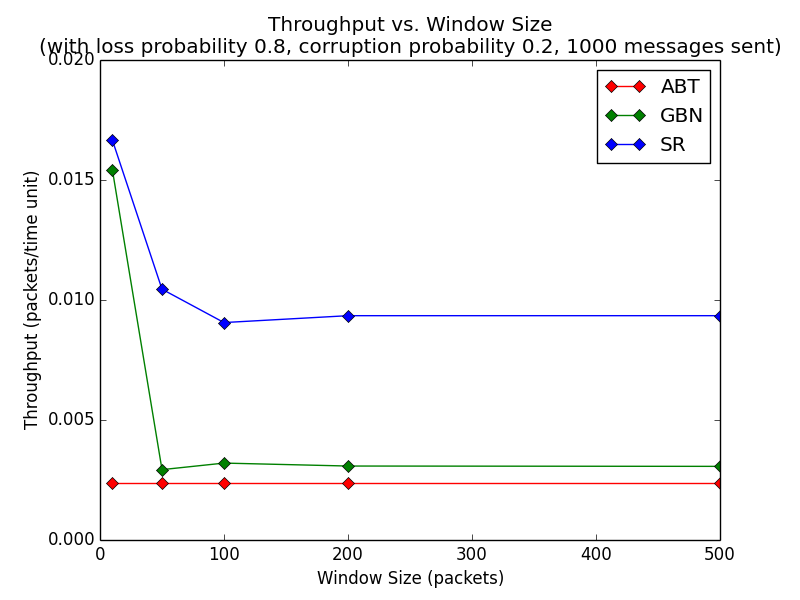
\includegraphics[width=330pt,height=245pt]{images/exp2g3.png}
\end{center}

\textbf{Expected}: Constant throughput for each protocol, but lower than than that of experiment (2b) due to increased packet loss.
\newline\newline
\textbf{Observed}: Constant throughput for ABT. Large drop of throughput for both GBN and SR with window size $\ge 10$. SR decisvely outperforms GBN in terms of throughput with window size $\ge 50$. Window size 10 offers the most throughput under this high packet loss scenario.
\newline\newline
\textbf{Conclusion}: The throughput of SR is more resilient than GBN and ABT under conditions of high packet loss. There exists an optimal window size for each protocol that maximizes throughput with a certain level of packet loss, in this case it is 10.

\pagebreak

\section{Conclusions Summarized}
\begin{enumerate}
    \item Increasing packet loss eventually decreases throughput in all three protocols.
    \item The throughput of both SR and GBN are more resilient to packet loss than ABT.
    \item The throughput of SR is more resilient to packet loss than both GBN and ABT.
    \item Under ideal conditions ($l=0.0, c=0.0$) a larger window size will increase throughput only if an application sends messages fast enough to fill the window.
    \item There exists an optimal window size that maximizes throughput under most packet loss conditions. Based on the experiments conducted, a window size of 50 would be a good choice for both SR and GBN. This window size allows for the most throughput under the most diverse range of conditions, while keeping memory usage on each endpoint minimal. However, this window size is optimal only in this specific scenario where the application is sending messages every 50 time units. In reality, this rate will be unpredictable. This suggests that it might be useful to potentially look into designing a new protocol based off SR or GBN that has a window size ``auto-tuning'' feature to maximize performance based on the sending rate of the application.
    \item From (1-5) SR is the protocol which offers the most throughput under the most diverse range of conditions, and is the more superior protocol in terms of performance.
\end{enumerate}
\end{document}
